\documentclass[a4paper]{article}

\usepackage{a4wide}
%\usepackage[french]{babel}
\usepackage[latin1,latin9,utf8,utf8x]{inputenc}
\usepackage[T1]{fontenc}
\usepackage{lmodern}
\usepackage{tikz}

\title{Corpus design for expressive speech: impact of the utterance length}
\author{Nelly Barbot \and Laurent Miclet \and Henri Prade}
\date{\today}

\begin{document}

\maketitle

\begin{abstract}
  Voice corpus plays a crucial role in the quality of the synthetic speech generation, specially under a length constraint. Creating a new voice is costly and the recording script selection for an expressive TTS task is generally considered as an optimization problem in order to achieve a rich and parsimonious corpus. In order to vocalize a given book using a TTS system, we investigate four script selection approaches. Based on preliminary observations, we simply propose to select shortest utterances of the book and compare the achievements of this method with state of the art ones for two books, with different utterance lengths and styles, using two kinds of concatenation based TTS systems. The study of the TTS costs indicates that selecting the shortest utterances could result in better synthetic quality, which is confirmed by a perceptual test. By investigating usual criteria for corpus design in literature like unit coverage or distribution similarity of units, it turns out that they are not pertinent metrics in the framework of this study. 
\end{abstract}
\foreach \n in{1,...,400}  {

\section{Ma section \n}

Lamque lituis cladium concrepantibus internarum non celate ut antea turbidum saeviebat ingenium a veri consideratione detortum et nullo inpositorum vel conpositorum fidem sollemniter inquirente nec discernente a societate noxiorum insontes velut exturbatum e iudiciis fas omne discessit, et causarum legitima silente defensione carnifex rapinarum sequester et obductio capitum et bonorum ubique multatio versabatur per orientales provincias, quas recensere puto nunc oportunum absque Mesopotamia digesta, cum bella Parthica dicerentur, et Aegypto, quam necessario aliud reieci ad tempus.

\foreach \s in{1,...,20}  {

\subsection{Ma sous section \s}

Sed ut tum ad senem senex de senectute, sic hoc libro ad amicum amicissimus scripsi de amicitia. Tum est Cato locutus, quo erat nemo fere senior temporibus illis, nemo prudentior; nunc Laelius et sapiens (sic enim est habitus) et amicitiae gloria excellens de amicitia loquetur. Tu velim a me animum parumper avertas, Laelium loqui ipsum putes. C. Fannius et Q. Mucius ad socerum veniunt post mortem Africani; ab his sermo oritur, respondet Laelius, cuius tota disputatio est de amicitia, quam legens te ipse cognosces.


\begin{figure}[htbp]
  \begin{center}
    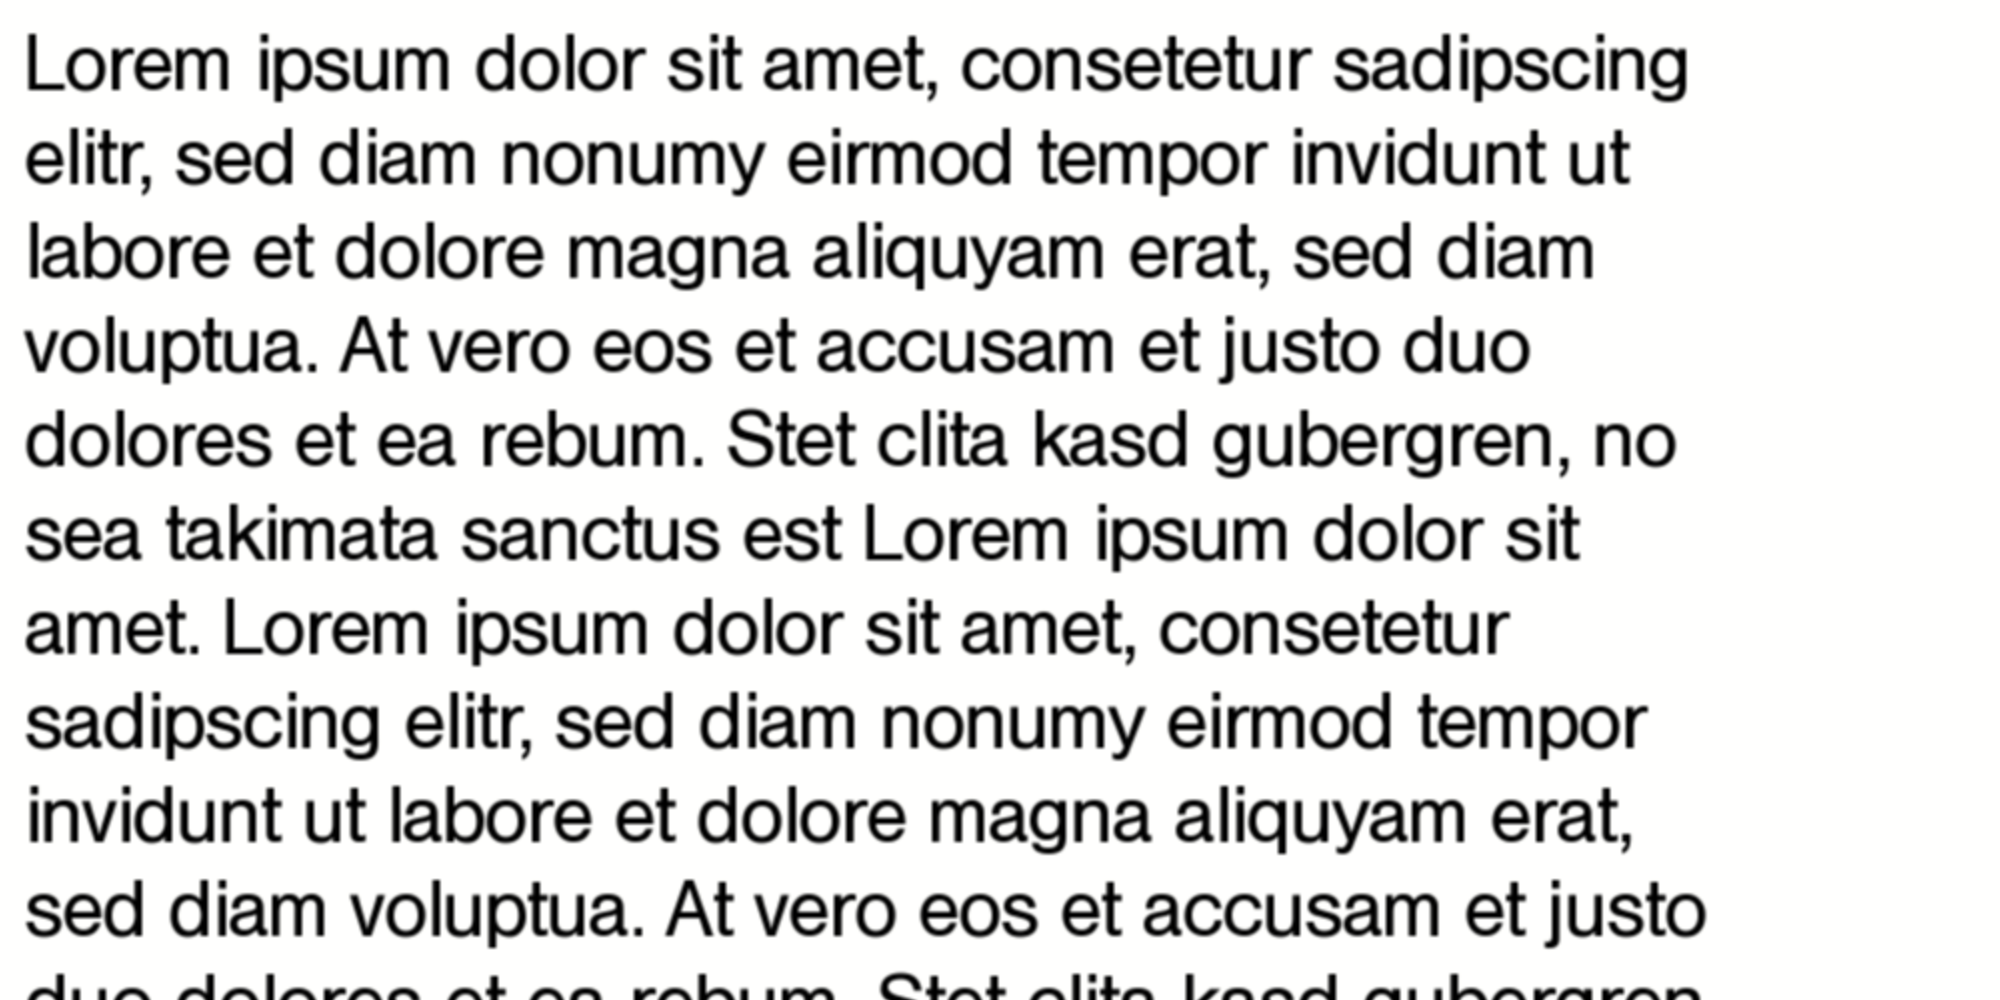
\includegraphics[width=.98\textwidth]{Que-signifie-Lorem-ipsum.png}
  \end{center}
  \caption{Lorem ipsum}
  \label{fig:1\s}
\end{figure}

Quapropter a natura mihi videtur potius quam ab indigentia orta amicitia, applicatione magis animi cum quodam sensu amandi quam cogitatione quantum illa res utilitatis esset habitura. Quod quidem quale sit, etiam in bestiis quibusdam animadverti potest, quae ex se natos ita amant ad quoddam tempus et ab eis ita amantur ut facile earum sensus appareat. Quod in homine multo est evidentius, primum ex ea caritate quae est inter natos et parentes, quae dirimi nisi detestabili scelere non potest; deinde cum similis sensus exstitit amoris, si aliquem nacti sumus cuius cum moribus et natura congruamus, quod in eo quasi lumen aliquod probitatis et virtutis perspicere videamur.

}

Martinus agens illas provincias pro praefectis aerumnas innocentium graviter gemens saepeque obsecrans, ut ab omni culpa inmunibus parceretur, cum non inpetraret, minabatur se discessurum: ut saltem id metuens perquisitor malivolus tandem desineret quieti coalitos homines in aperta pericula proiectare.

Sed laeditur hic coetuum magnificus splendor levitate paucorum incondita, ubi nati sunt non reputantium, sed tamquam indulta licentia vitiis ad errores lapsorum ac lasciviam. ut enim Simonides lyricus docet, beate perfecta ratione vieturo ante alia patriam esse convenit gloriosam.

\begin{figure}[htbp]
  \begin{center}
    
\includegraphics[width=.98\textwidth]{Lorem_ipsum_flush_justified.png}
  \end{center}
  \caption{Lorem ipsum}
  \label{fig:3}
\end{figure}


Quam ob rem circumspecta cautela observatum est deinceps et cum edita montium petere coeperint grassatores, loci iniquitati milites cedunt. ubi autem in planitie potuerint reperiri, quod contingit adsidue, nec exsertare lacertos nec crispare permissi tela, quae vehunt bina vel terna, pecudum ritu inertium trucidantur.

\foreach \t in{1,...,20}  {

\subsection{Ma sous section \t}

Accedebant enim eius asperitati, ubi inminuta vel laesa amplitudo imperii dicebatur, et iracundae suspicionum quantitati proximorum cruentae blanditiae exaggerantium incidentia et dolere inpendio simulantium, si principis periclitetur vita, a cuius salute velut filo pendere statum orbis terrarum fictis vocibus exclamabant.

\begin{figure}[htbp]
  \begin{center}
    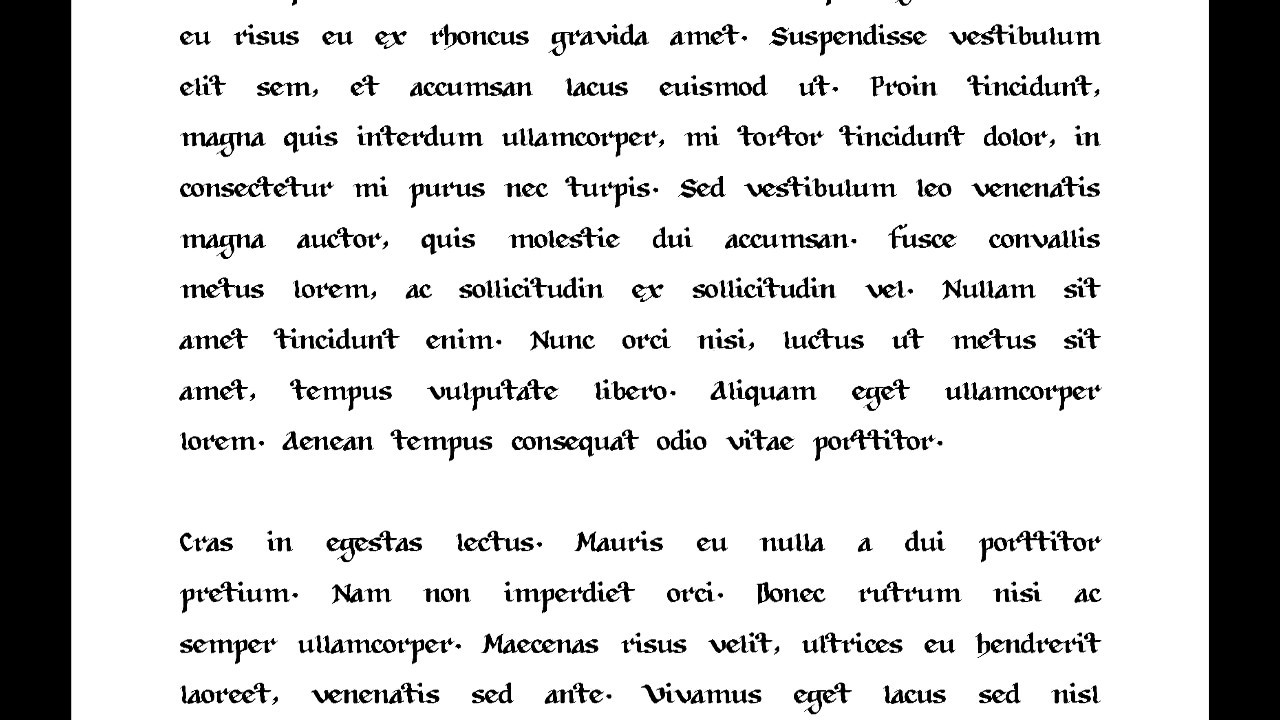
\includegraphics[width=.98\textwidth]{maxresdefault.jpg}
  \end{center}
  \caption{Lorem ipsum}
  \label{fig:4\t}
\end{figure}

Iamque lituis cladium concrepantibus internarum non celate ut antea turbidum saeviebat ingenium a veri consideratione detortum et nullo inpositorum vel conpositorum fidem sollemniter inquirente nec discernente a societate noxiorum insontes velut exturbatum e iudiciis fas omne discessit, et causarum legitima silente defensione carnifex rapinarum sequester et obductio capitum et bonorum ubique multatio versabatur per orientales provincias, quas recensere puto nunc oportunum absque Mesopotamia digesta, cum bella Parthica dicerentur, et Aegypto, quam necessario aliud reieci ad tempus.

}
Quapropter a natura mihi videtur potius quam ab indigentia orta amicitia, applicatione magis animi cum quodam sensu amandi quam cogitatione quantum illa res utilitatis esset habitura. Quod quidem quale sit, etiam in bestiis quibusdam animadverti potest, quae ex se natos ita amant ad quoddam tempus et ab eis ita amantur ut facile earum sensus appareat. Quod in homine multo est evidentius, primum ex ea caritate quae est inter natos et parentes, quae dirimi nisi detestabili scelere non potest; deinde cum similis sensus exstitit amoris, si aliquem nacti sumus cuius cum moribus et natura congruamus, quod in eo quasi lumen aliquod probitatis et virtutis perspicere videamur.

Vita est illis semper in fuga uxoresque mercenariae conductae ad tempus ex pacto atque, ut sit species matrimonii, dotis nomine futura coniunx hastam et tabernaculum offert marito, post statum diem si id elegerit discessura, et incredibile est quo ardore apud eos in venerem uterque solvitur sexus.

\begin{figure}[htbp]
  \begin{center}
    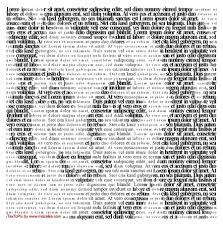
\includegraphics[width=.98\textwidth]{index.jpeg}
  \end{center}
  \caption{Lorem ipsum}
  \label{fig:5}
\end{figure}

Cum autem commodis intervallata temporibus convivia longa et noxia coeperint apparari vel distributio sollemnium sportularum, anxia deliberatione tractatur an exceptis his quibus vicissitudo debetur, peregrinum invitari conveniet, et si digesto plene consilio id placuerit fieri, is adhibetur qui pro domibus excubat aurigarum aut artem tesserariam profitetur aut secretiora quaedam se nosse confingit.

Accenderat super his incitatum propositum ad nocendum aliqua mulier vilis, quae ad palatium ut poposcerat intromissa insidias ei latenter obtendi prodiderat a militibus obscurissimis. quam Constantina exultans ut in tuto iam locata mariti salute muneratam vehiculoque inpositam per regiae ianuas emisit in publicum, ut his inlecebris alios quoque ad indicanda proliceret paria vel maiora.

Tempore quo primis auspiciis in mundanum fulgorem surgeret victura dum erunt homines Roma, ut augeretur sublimibus incrementis, foedere pacis aeternae Virtus convenit atque Fortuna plerumque dissidentes, quarum si altera defuisset, ad perfectam non venerat summitatem.

Exsistit autem hoc loco quaedam quaestio subdifficilis, num quando amici novi, digni amicitia, veteribus sint anteponendi, ut equis vetulis teneros anteponere solemus. Indigna homine dubitatio! Non enim debent esse amicitiarum sicut aliarum rerum satietates; veterrima quaeque, ut ea vina, quae vetustatem ferunt, esse debet suavissima; verumque illud est, quod dicitur, multos modios salis simul edendos esse, ut amicitiae munus expletum sit.

Proinde die funestis interrogationibus praestituto imaginarius iudex equitum resedit magister adhibitis aliis iam quae essent agenda praedoctis, et adsistebant hinc inde notarii, quid quaesitum esset, quidve responsum, cursim ad Caesarem perferentes, cuius imperio truci, stimulis reginae exsertantis aurem subinde per aulaeum, nec diluere obiecta permissi nec defensi periere conplures.

Has autem provincias, quas Orontes ambiens amnis imosque pedes Cassii montis illius celsi praetermeans funditur in Parthenium mare, Gnaeus Pompeius superato Tigrane regnis Armeniorum abstractas dicioni Romanae coniunxit.

Fuerit toto in consulatu sine provincia, cui fuerit, antequam designatus est, decreta provincia. Sortietur an non? Nam et non sortiri absurdum est, et, quod sortitus sis, non habere. Proficiscetur paludatus? Quo? Quo pervenire ante certam diem non licebit. ianuario, Februario, provinciam non habebit; Kalendis ei denique Martiis nascetur repente provincia.

\begin{figure}[htbp]
  \begin{center}
    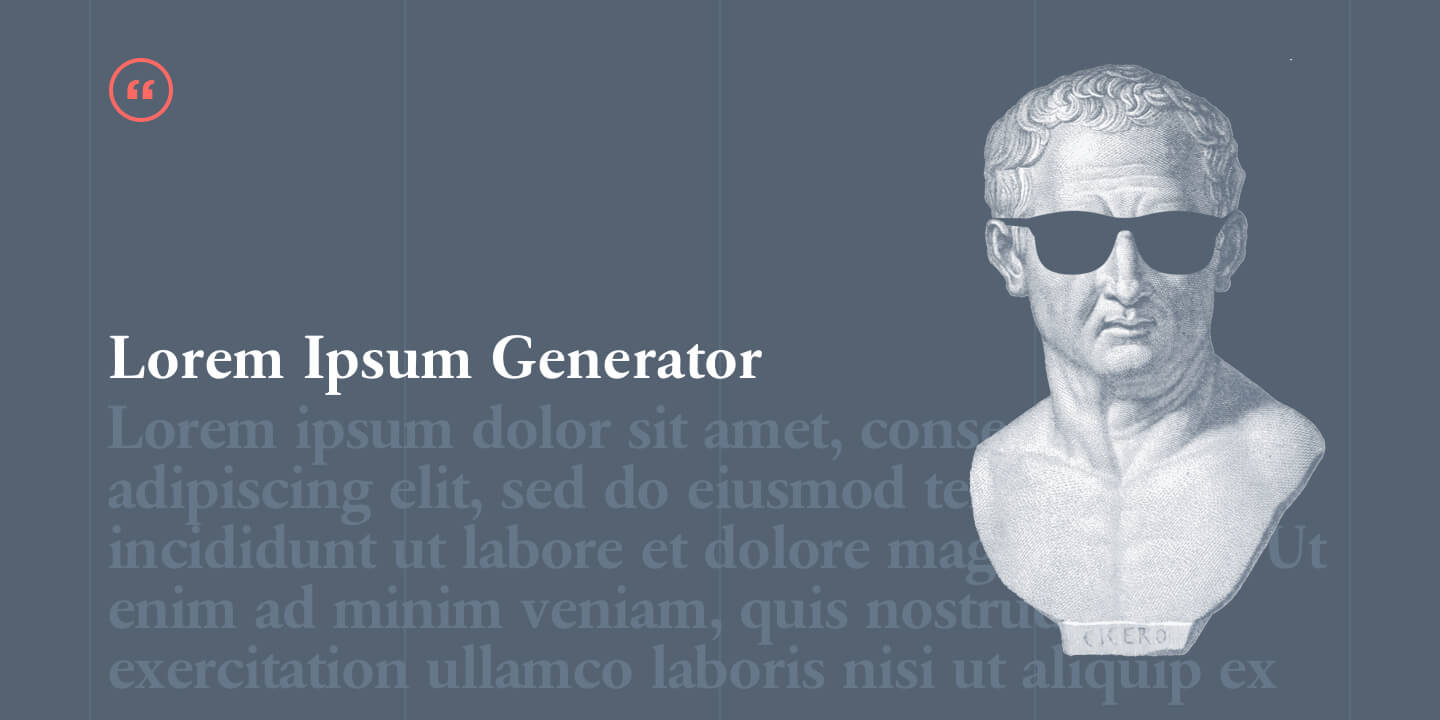
\includegraphics[width=.98\textwidth]{lorem-ipsum-generator-custom-placeholder-text.jpg}
  \end{center}
  \caption{Lorem ipsum}
  \label{fig:2}
\end{figure}

Principium autem unde latius se funditabat, emersit ex negotio tali. Chilo ex vicario et coniux eius Maxima nomine, questi apud Olybrium ea tempestate urbi praefectum, vitamque suam venenis petitam adseverantes inpetrarunt ut hi, quos suspectati sunt, ilico rapti conpingerentur in vincula, organarius Sericus et Asbolius palaestrita et aruspex Campensis.

Isdem diebus Apollinaris Domitiani gener, paulo ante agens palatii Caesaris curam, ad Mesopotamiam missus a socero per militares numeros immodice scrutabatur, an quaedam altiora meditantis iam Galli secreta susceperint scripta, qui conpertis Antiochiae gestis per minorem Armeniam lapsus Constantinopolim petit exindeque per protectores retractus artissime tenebatur.

Et olim licet otiosae sint tribus pacataeque centuriae et nulla suffragiorum certamina set Pompiliani redierit securitas temporis, per omnes tamen quotquot sunt partes terrarum, ut domina suscipitur et regina et ubique patrum reverenda cum auctoritate canities populique Romani nomen circumspectum et verecundum.


}
\end{document}
